\documentclass[12pt,letterpaper]{article}\usepackage[]{graphicx}\usepackage[]{color}
%% maxwidth is the original width if it is less than linewidth
%% otherwise use linewidth (to make sure the graphics do not exceed the margin)
\makeatletter
\def\maxwidth{ %
  \ifdim\Gin@nat@width>\linewidth
    \linewidth
  \else
    \Gin@nat@width
  \fi
}
\makeatother

\definecolor{fgcolor}{rgb}{0.345, 0.345, 0.345}
\newcommand{\hlnum}[1]{\textcolor[rgb]{0.686,0.059,0.569}{#1}}%
\newcommand{\hlstr}[1]{\textcolor[rgb]{0.192,0.494,0.8}{#1}}%
\newcommand{\hlcom}[1]{\textcolor[rgb]{0.678,0.584,0.686}{\textit{#1}}}%
\newcommand{\hlopt}[1]{\textcolor[rgb]{0,0,0}{#1}}%
\newcommand{\hlstd}[1]{\textcolor[rgb]{0.345,0.345,0.345}{#1}}%
\newcommand{\hlkwa}[1]{\textcolor[rgb]{0.161,0.373,0.58}{\textbf{#1}}}%
\newcommand{\hlkwb}[1]{\textcolor[rgb]{0.69,0.353,0.396}{#1}}%
\newcommand{\hlkwc}[1]{\textcolor[rgb]{0.333,0.667,0.333}{#1}}%
\newcommand{\hlkwd}[1]{\textcolor[rgb]{0.737,0.353,0.396}{\textbf{#1}}}%

\usepackage{framed}
\makeatletter
\newenvironment{kframe}{%
 \def\at@end@of@kframe{}%
 \ifinner\ifhmode%
  \def\at@end@of@kframe{\end{minipage}}%
  \begin{minipage}{\columnwidth}%
 \fi\fi%
 \def\FrameCommand##1{\hskip\@totalleftmargin \hskip-\fboxsep
 \colorbox{shadecolor}{##1}\hskip-\fboxsep
     % There is no \\@totalrightmargin, so:
     \hskip-\linewidth \hskip-\@totalleftmargin \hskip\columnwidth}%
 \MakeFramed {\advance\hsize-\width
   \@totalleftmargin\z@ \linewidth\hsize
   \@setminipage}}%
 {\par\unskip\endMakeFramed%
 \at@end@of@kframe}
\makeatother

\definecolor{shadecolor}{rgb}{.97, .97, .97}
\definecolor{messagecolor}{rgb}{0, 0, 0}
\definecolor{warningcolor}{rgb}{1, 0, 1}
\definecolor{errorcolor}{rgb}{1, 0, 0}
\newenvironment{knitrout}{}{} % an empty environment to be redefined in TeX

\usepackage{alltt}
 \usepackage[left=2cm,right=2cm,top=2cm,bottom=2cm]{geometry}
\usepackage[ansinew]{inputenc}
\usepackage[spanish]{babel}
\usepackage{amsmath}
\usepackage{amsfonts}
\usepackage{amssymb}
\usepackage{dsfont}
\usepackage{multicol} 
\usepackage{subfigure}
\usepackage{graphicx}
\usepackage{float} 
\usepackage{verbatim} 
\usepackage[left=2cm,right=2cm,top=2cm,bottom=2cm]{geometry}
\usepackage{fancyhdr}
\pagestyle{fancy} 
\fancyhead[LO]{\leftmark}
\usepackage{caption}
\newtheorem{definicion}{Definci\'on}
\IfFileExists{upquote.sty}{\usepackage{upquote}}{}
\begin{document}

\begin{titlepage}
\setlength{\unitlength}{1 cm} %Especificar unidad de trabajo


\begin{center}
\textbf{{\large UNIVERSIDAD DE EL SALVADOR}\\
{\large FACULTAD MULTIDISCIPLINARIA DE OCCIDENTE}\\
{\large DEPARTAMENTO DE MATEM\'ATICA}}\\[0.50 cm]

\begin{picture}(18,4)
 \put(7,0){
\includegraphics[width=4cm]{minerva.jpg}}
\end{picture}
\\[0.25 cm]

\textbf{{\large Licenciatura en Estad\'istica}\\[1.25cm]
{\large Control Estadistico del Paquete R }\\[2 cm]
%\setlength{\unitlength}{1 cm}
{\large  \textbf{''UNIDAD DOS"}}\\
{\large  \textbf{PR\'ACTICA 06 - AN\'ALISIS DE DATOS CATEG\'ORICOS.}}\\[3 cm]
{\large Alumna:}\\
{\large Martha Yoana Medina S\'anchez}\\[2cm]
{\large Fecha de elaboraci\'on}\\
Santa Ana - \today }
\end{center}
\end{titlepage}

\newtheorem{teorema}{Teorema}
\newtheorem{prop}{Proposici\'on}[section]

\lhead{UNIDAD DOS}
\chead{PRACTICA 06}
\lfoot{LICENCIATURA EN ESTAD\'ISTICA}
\cfoot{UESOCC}
\rfoot{\thepage}
%\pagestyle{fancy} 

\setcounter{page}{1}
\newpage

\begin{center}
\textbf{Pr\'actica 06 - An\'alisis de datos categ\'oricos.}
\end{center}

\begin{center}
\textbf{ESCALAS DE MEDICI\'ON}\\
\end{center}

Como la estad\'istica analiza los datos y \'estos son producto de las mediciones, necesitamos estudiar las escalas de medici\'on. Este tema es de suma importancia, pues el tipo de escala de medici\'on utilizado para reunir los datos ayuda a determinar el tipo de an\'alisis a utilizar en los datos. Existen cuatro clases de escalas que aparecen de manera com\'un en las ciencias: nominal, ordinal, de intervalo y de raz\'on. Ellas difieren en el n\'umero de atributos matem\'aticos que poseen.\\


Los tipos de datos univariados que vamos a analizar en esta pr\'actica son:\\

\textbf{Categ\'oricos.}Tienen la caracter\'istica de que todos los miembros de una categor\'ia se consideran iguales en lo que se refiere a ese tipo. Este tipode datos se subdivide en nominales y ordinales.

\begin{itemize}
  \item \textbf{Nominales.}Los valores que pueden asumir sirven para clasificarlos pero no para ordenarlos. En caso de usarse n\'umeros, s\'olose adoptan como nombres o identificaciones.
  \item \textbf{Ordinales.}Los valores que puede asumir este tipo de datos son categor\'ias que conllevan un juicio de valor que exige comparar a los diferentes elementos de la muestra con respecto a este tipo con el objeto de establecer un orden. Es decir, que los datos se organizan a trav\'es de las relaciones de igualdad, mayor o menor. 
\end{itemize}
\begin{center}
  \textbf{1. AN\'ALISIS ESTAD\'ISTICO DE DATOS CATEG\'ORICOS.}
\end{center}

Ejemplo: Se realiza un estudio para conocer las preferencias sobre el tipo de gaseosa que se consume: \textbf{CC$=$Coca Cola, PC$=$Pepsi Cola, SC$=$Salva Cola}, para ello se toma una muestra aleatoria de 20 personas.\\

\begin{enumerate}
  \item  Activar el directorio de trabajo.

\begin{knitrout}
\definecolor{shadecolor}{rgb}{0.969, 0.969, 0.969}\color{fgcolor}\begin{kframe}
\begin{alltt}
\hlkwd{getwd}\hlstd{()}
\end{alltt}
\begin{verbatim}
## [1] "C:/Users/User/Documents/PRACTICAS_YOANA_MEDINA/Yoana/PRACTICAS DE R"
\end{verbatim}
\end{kframe}
\end{knitrout}
\begin{knitrout}
\definecolor{shadecolor}{rgb}{0.969, 0.969, 0.969}\color{fgcolor}\begin{kframe}
\begin{alltt}
\hlkwd{setwd}\hlstd{(}\hlstr{"C:/Users/User/Documents/PRACTICAS_YOANA_MEDINA/Yoana/PRACTICAS DE R"}\hlstd{)}
\end{alltt}
\end{kframe}
\end{knitrout}

\item  Crear un nuevo script y llamarle Script06-DatosCategoricos.

\item Crear un vector con el tipo de gaseosa y otro con la muestra generada aleatoriamente:
\begin{knitrout}
\definecolor{shadecolor}{rgb}{0.969, 0.969, 0.969}\color{fgcolor}\begin{kframe}
\begin{alltt}
\hlstd{Tipo} \hlkwb{<-} \hlkwd{c}\hlstd{(}\hlstr{"CC"}\hlstd{,} \hlstr{"PC"}\hlstd{,} \hlstr{"SC"}\hlstd{); Tipo}
\end{alltt}
\begin{verbatim}
## [1] "CC" "PC" "SC"
\end{verbatim}
\begin{alltt}
\hlcom{# crea un vector en las que contiene los tres tipos de refrescos}
\end{alltt}
\end{kframe}
\end{knitrout}
\begin{knitrout}
\definecolor{shadecolor}{rgb}{0.969, 0.969, 0.969}\color{fgcolor}\begin{kframe}
\begin{alltt}
\hlstd{Consumo} \hlkwb{<-} \hlkwd{sample}\hlstd{(Tipo,} \hlnum{20}\hlstd{,} \hlkwc{replace}\hlstd{=}\hlnum{TRUE}\hlstd{); Consumo}
\end{alltt}
\begin{verbatim}
##  [1] "PC" "PC" "SC" "PC" "PC" "CC" "PC" "CC" "CC" "SC" "PC" "PC" "SC" "CC"
## [15] "SC" "SC" "PC" "PC" "CC" "SC"
\end{verbatim}
\begin{alltt}
\hlcom{# genera una muestra de tamano 20 obtenida de los elementos del vector}
\hlcom{# Tipo y los elementos se seleccionan con reemplazamiento.}

\hlcom{# Suponiendo que se quiere editar o agregar datos }
\end{alltt}
\end{kframe}
\end{knitrout}
\begin{knitrout}
\definecolor{shadecolor}{rgb}{0.969, 0.969, 0.969}\color{fgcolor}\begin{kframe}
\begin{alltt}
\hlkwd{data.entry}\hlstd{(Consumo)}
\end{alltt}
\end{kframe}
\end{knitrout}

\item Guarde el vector en un archivo de datos
\begin{knitrout}
\definecolor{shadecolor}{rgb}{0.969, 0.969, 0.969}\color{fgcolor}\begin{kframe}
\begin{alltt}
\hlcom{# Guardar los datos en su directorio de trabajo }
\hlkwd{write}\hlstd{(Consumo,} \hlstr{"Consumo.txt"}\hlstd{)}
\end{alltt}
\end{kframe}
\end{knitrout}

\item Eliminar los objetos que existen en el espacio de trabajo (Workspace)
\begin{knitrout}
\definecolor{shadecolor}{rgb}{0.969, 0.969, 0.969}\color{fgcolor}\begin{kframe}
\begin{alltt}
\hlkwd{ls}\hlstd{()}
\end{alltt}
\begin{verbatim}
## [1] "Consumo" "Tipo"
\end{verbatim}
\begin{alltt}
\hlkwd{rm}\hlstd{(}\hlkwc{list}\hlstd{=}\hlkwd{ls}\hlstd{(}\hlkwc{all}\hlstd{=}\hlnum{TRUE}\hlstd{))}
\hlkwd{ls}\hlstd{()}
\end{alltt}
\begin{verbatim}
## character(0)
\end{verbatim}
\end{kframe}
\end{knitrout}

\item Leer o recuperar el vector de datos o archivo de texto 
\begin{knitrout}
\definecolor{shadecolor}{rgb}{0.969, 0.969, 0.969}\color{fgcolor}\begin{kframe}
\begin{alltt}
\hlstd{Consumo} \hlkwb{<-} \hlkwd{scan}\hlstd{(}\hlstr{"Consumo.txt"}\hlstd{,} \hlkwc{what}\hlstd{=} \hlkwd{character}\hlstd{(),} \hlkwc{na.strings} \hlstd{=} \hlstr{"NA"}\hlstd{,}
\hlkwc{flush}\hlstd{=}\hlnum{FALSE}\hlstd{);Consumo}
\end{alltt}
\begin{verbatim}
##  [1] "PC" "PC" "SC" "PC" "PC" "CC" "PC" "CC" "CC" "SC" "PC" "PC" "SC" "CC"
## [15] "SC" "SC" "PC" "PC" "CC" "SC"
\end{verbatim}
\begin{alltt}
\hlkwd{ls}\hlstd{()}
\end{alltt}
\begin{verbatim}
## [1] "Consumo"
\end{verbatim}
\begin{alltt}
\hlcom{# Si el vector contiene caracteresse ocupa: what = character() }
\hlcom{# na.strings ="NA", le indica a R que los valores faltantes son identificados}
\hlcom{# con "NA" }
\end{alltt}
\end{kframe}
\end{knitrout}

\item  Crear la tabla de distribuci\'on de frecuencias y proporciones
\begin{knitrout}
\definecolor{shadecolor}{rgb}{0.969, 0.969, 0.969}\color{fgcolor}\begin{kframe}
\begin{alltt}
\hlstd{frec} \hlkwb{<-} \hlkwd{table}\hlstd{(Consumo); frec}
\end{alltt}
\begin{verbatim}
## Consumo
## CC PC SC 
##  5  9  6
\end{verbatim}
\begin{alltt}
\hlstd{prop} \hlkwb{<-} \hlkwd{table}\hlstd{(Consumo)}\hlopt{/}\hlkwd{length}\hlstd{(Consumo); prop}
\end{alltt}
\begin{verbatim}
## Consumo
##   CC   PC   SC 
## 0.25 0.45 0.30
\end{verbatim}
\begin{alltt}
\hlcom{# Note que la salida por defecto no es para nada atractiva en comparacion con }
\hlcom{# el resto de paquetes estadisticos }
\end{alltt}
\end{kframe}
\end{knitrout}
\begin{knitrout}
\definecolor{shadecolor}{rgb}{0.969, 0.969, 0.969}\color{fgcolor}\begin{kframe}
\begin{alltt}
\hlcom{# En cambio, si estamos usando LATEX y queremos incorporar estos cuadros o}
\hlcom{# cualquier otro podemos utilizar el comando xtable(table(Consumo)) (NOTE }
\hlcom{# QUE EL ARGUMENTO DEBE SER UN CUADRO), y con esto automaticamente se nos }
\hlcom{# genera el codigo en LATEX y luego incorporarlo a nuestro informe, lo mejor}
\hlcom{# de todo es que salida resultante es mucho mas presentable. }
\end{alltt}
\end{kframe}
\end{knitrout}

\item  Conocer un resumen de los datos 
\begin{knitrout}
\definecolor{shadecolor}{rgb}{0.969, 0.969, 0.969}\color{fgcolor}\begin{kframe}
\begin{alltt}
\hlkwd{summary}\hlstd{(Consumo)}
\end{alltt}
\begin{verbatim}
##    Length     Class      Mode 
##        20 character character
\end{verbatim}
\begin{alltt}
\hlcom{# note que por tratarse de variables cualitativas unicamente muestra el }
\hlcom{# numero de elementos, y el tipo de datos. }
\end{alltt}
\end{kframe}
\end{knitrout}

\item Realizar un gr\'afico de barras
\begin{knitrout}
\definecolor{shadecolor}{rgb}{0.969, 0.969, 0.969}\color{fgcolor}\begin{kframe}
\begin{alltt}
\hlcom{# Para las frecuencias absolutas }
\hlkwd{barplot}\hlstd{(frec,} \hlkwc{main}\hlstd{=}\hlstr{"Grafico de barras"}\hlstd{,}
        \hlkwc{xlab}\hlstd{=}\hlstr{"Consumo"}\hlstd{,} \hlkwc{col}\hlstd{=}\hlkwd{c}\hlstd{(}\hlstr{"yellow"}\hlstd{,} \hlstr{"white"}\hlstd{,} \hlstr{"red"}\hlstd{),}
        \hlkwc{sub}\hlstd{=}\hlstr{"Agosto-2012"}\hlstd{)}
\end{alltt}
\end{kframe}
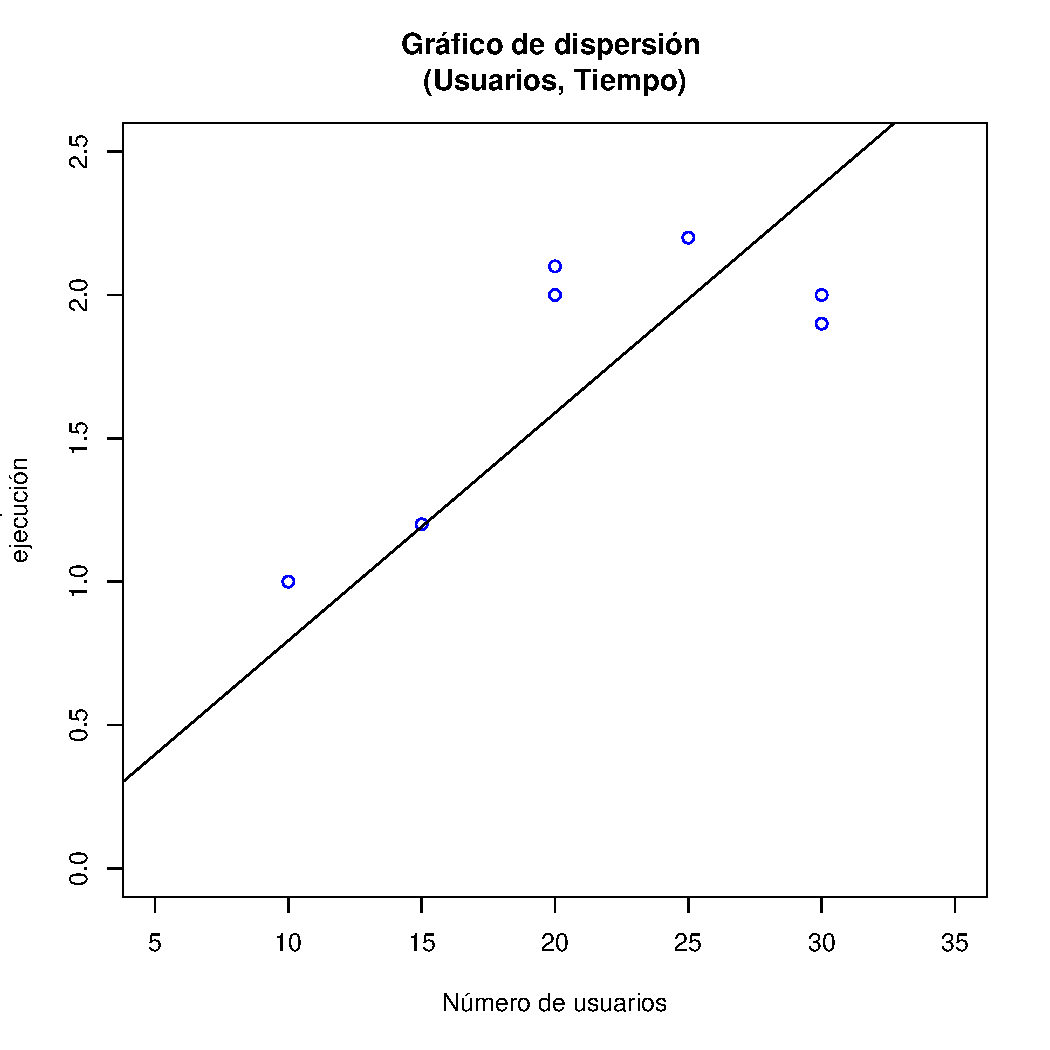
\includegraphics[width=\maxwidth]{figure/unnamed-chunk-12-1} 
\begin{kframe}\begin{alltt}
\hlcom{# Para las frecuencias relativas }
\hlkwd{barplot}\hlstd{(prop,} \hlkwc{main}\hlstd{=}\hlstr{"Grafico de barras"}\hlstd{,} \hlkwc{xlab}\hlstd{=}\hlstr{" Consumo\textbackslash{}n"}\hlstd{,}
        \hlkwc{col}\hlstd{=}\hlkwd{c}\hlstd{(}\hlstr{"yellow"}\hlstd{,}\hlstr{"white"}\hlstd{,} \hlstr{"red"}\hlstd{),}
        \hlkwc{sub}\hlstd{=}\hlstr{"Agosto-2012"}\hlstd{)}
\end{alltt}
\end{kframe}
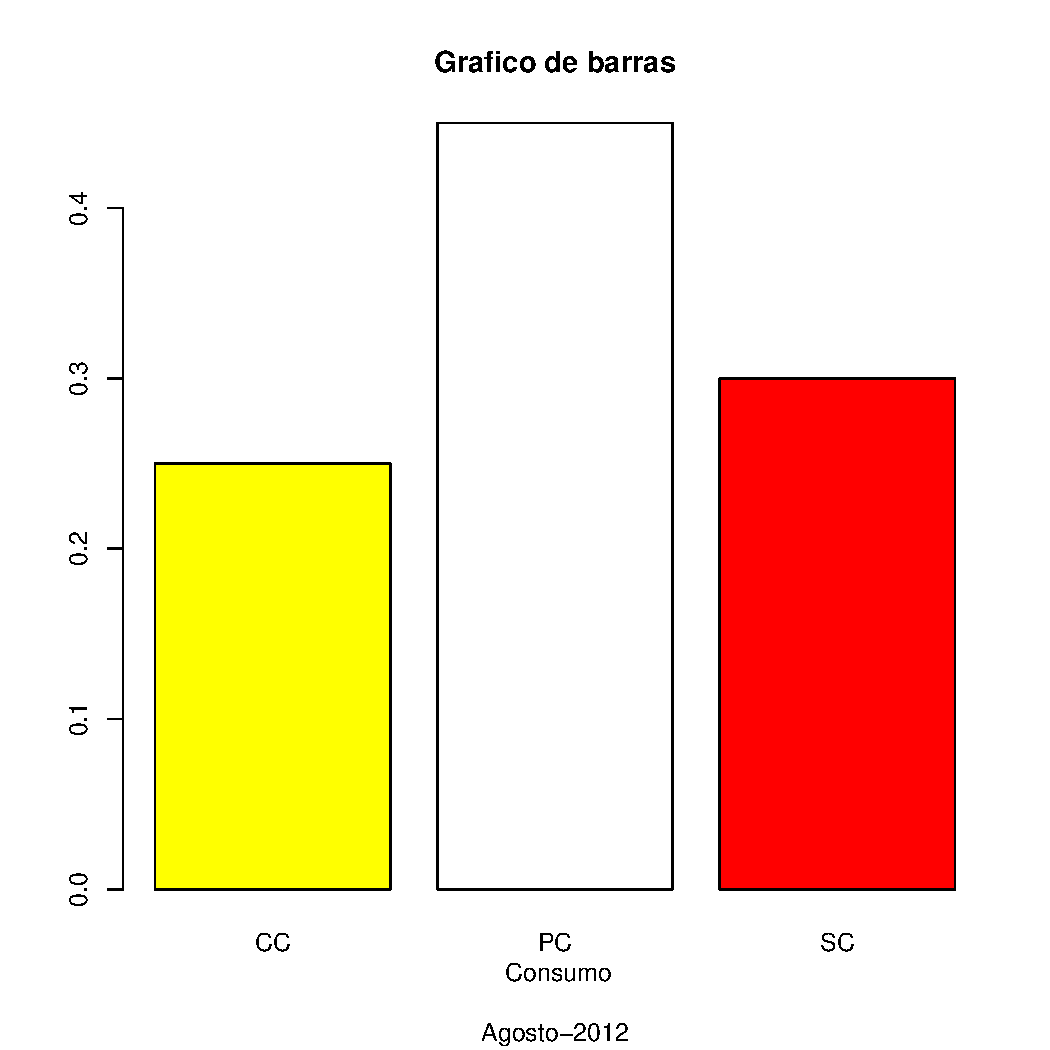
\includegraphics[width=\maxwidth]{figure/unnamed-chunk-12-2} 

\end{knitrout}

\item Realizar un gr\'afico de pastel 
\begin{knitrout}
\definecolor{shadecolor}{rgb}{0.969, 0.969, 0.969}\color{fgcolor}\begin{kframe}
\begin{alltt}
\hlkwd{pie}\hlstd{(frec,} \hlkwc{main}\hlstd{=}\hlstr{"Gráfico de pastel"}\hlstd{,} \hlkwc{xlab}\hlstd{=}\hlstr{"Tipo de Consumo"}\hlstd{,}
    \hlkwc{col}\hlstd{=}\hlkwd{c}\hlstd{(}\hlstr{"yellow"}\hlstd{,} \hlstr{"white"}\hlstd{,} \hlstr{"cyan"}\hlstd{),} \hlkwc{sub}\hlstd{=}\hlstr{"Agosto-2012"}\hlstd{)}
\end{alltt}
\end{kframe}
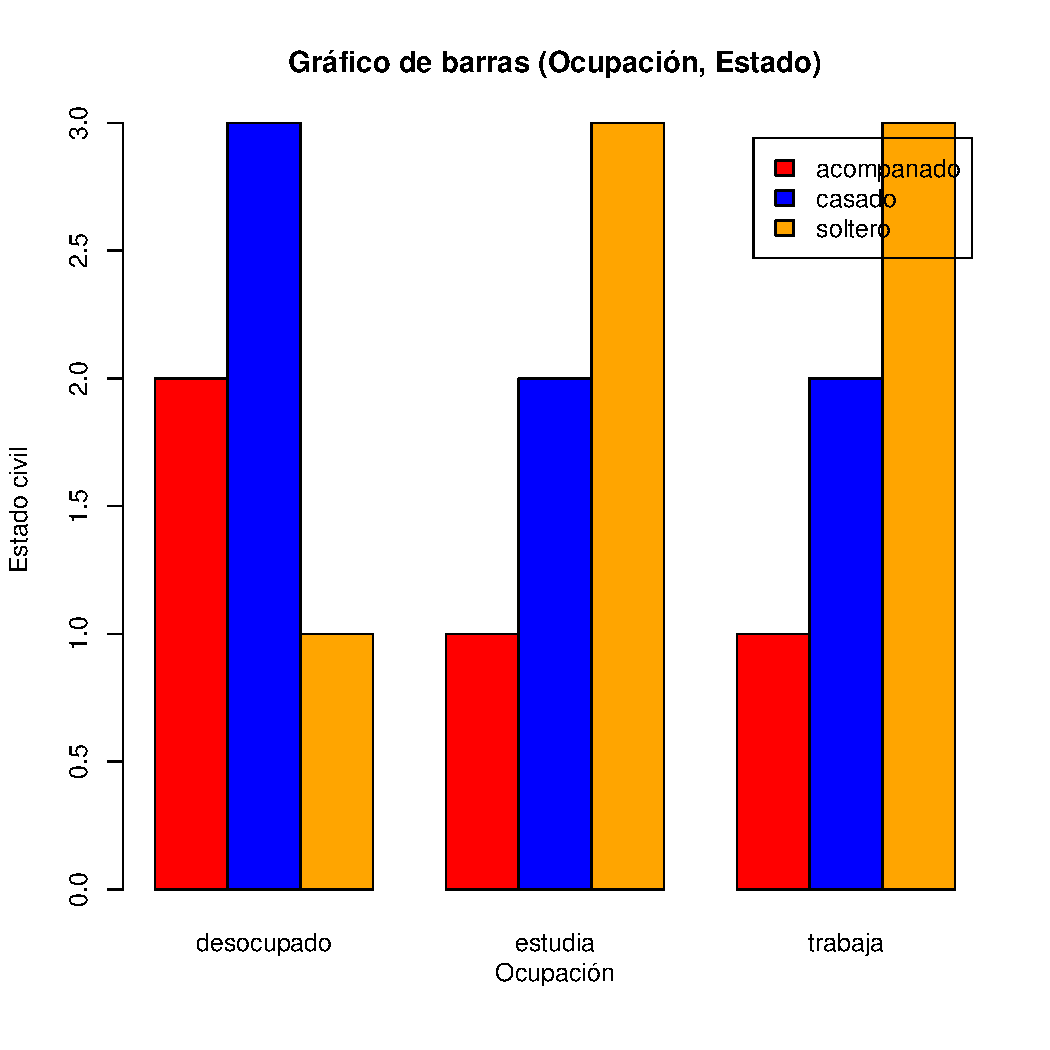
\includegraphics[width=\maxwidth]{figure/unnamed-chunk-13-1} 

\end{knitrout}
\begin{knitrout}
\definecolor{shadecolor}{rgb}{0.969, 0.969, 0.969}\color{fgcolor}\begin{kframe}
\begin{alltt}
\hlcom{# Se puede especificar nombres para las categorias y el color de los sectores}

\hlkwd{names}\hlstd{(frec)} \hlkwb{=} \hlkwd{c}\hlstd{(}\hlstr{"Coca Cola"}\hlstd{,} \hlstr{"Pepsi"}\hlstd{,} \hlstr{"Salva Cola"}\hlstd{)}
\hlkwd{pie}\hlstd{(frec,} \hlkwc{main}\hlstd{=}\hlstr{"Gráfico de pastel"}\hlstd{,} \hlkwc{xlab}\hlstd{=}\hlstr{" Consumo"}\hlstd{,} \hlkwc{radius}\hlstd{=}\hlnum{0.8}\hlstd{,}
    \hlkwc{col}\hlstd{=}\hlkwd{c}\hlstd{(}\hlstr{"red"}\hlstd{,} \hlstr{"gray"}\hlstd{,} \hlstr{"cyan"}\hlstd{),} \hlkwc{sub}\hlstd{=}\hlstr{"Agosto-2012"}\hlstd{)}
\end{alltt}
\end{kframe}
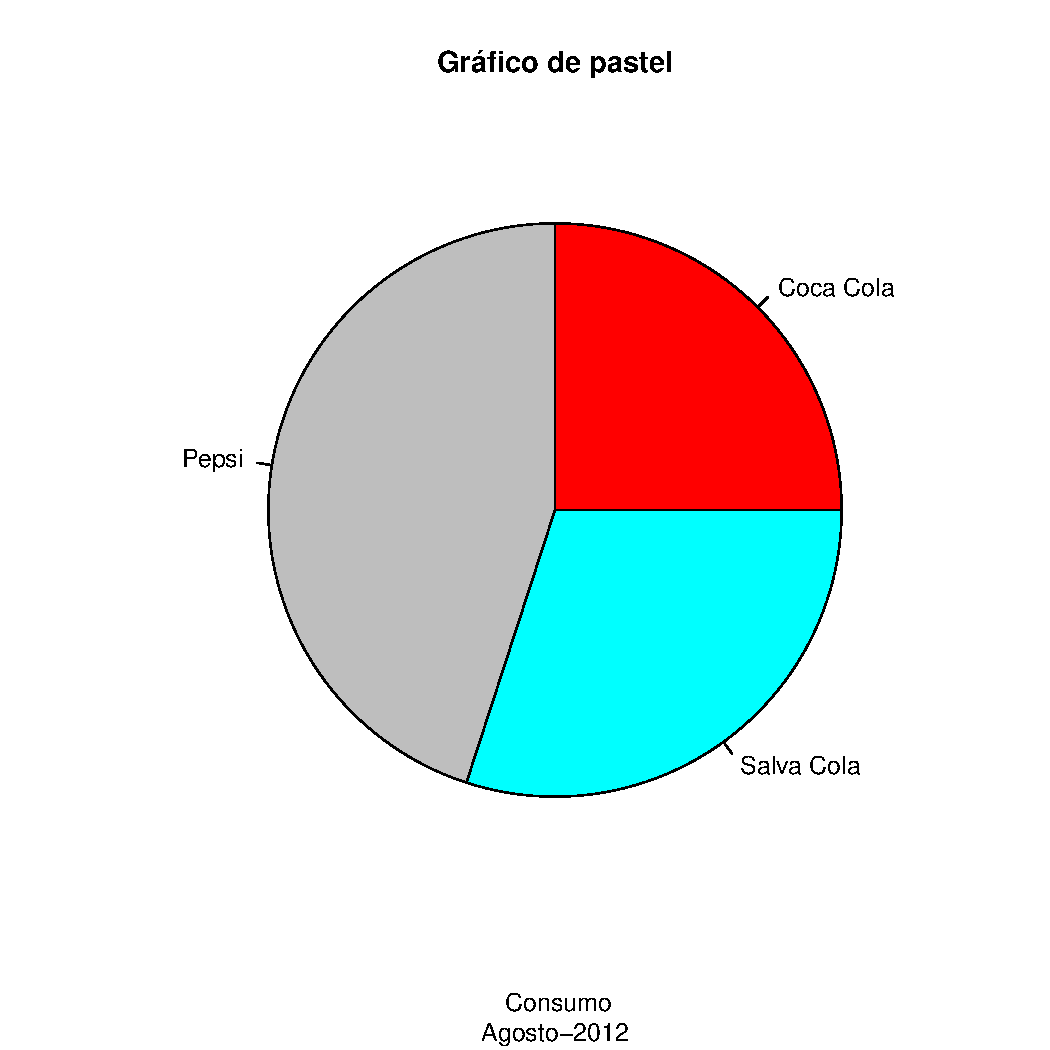
\includegraphics[width=\maxwidth]{figure/unnamed-chunk-14-1} 
\begin{kframe}\begin{alltt}
\hlcom{# Los colores se asignas dependiendo del orden en que han sido especificados }
\hlcom{# por names()}

\hlcom{# Note con la instrucción radius se especifica el tamaño de la figura, mientras}
\hlcom{# mas cerca de uno (uno de menos uno) se encuentre más grande será (el ángulo}
\hlcom{# cambia). }
\end{alltt}
\end{kframe}
\end{knitrout}

\item Colocar valores num\'ericos en los sectores del gr\'afico
\begin{knitrout}
\definecolor{shadecolor}{rgb}{0.969, 0.969, 0.969}\color{fgcolor}\begin{kframe}
\begin{alltt}
\hlstd{n} \hlkwb{<-} \hlkwd{length}\hlstd{(frec)}
\hlstd{hoja} \hlkwb{<-} \hlkwd{data.frame}\hlstd{(frec); hoja}
\end{alltt}
\begin{verbatim}
##         Var1 Freq
## 1  Coca Cola    5
## 2      Pepsi    9
## 3 Salva Cola    6
\end{verbatim}
\begin{alltt}
\hlstd{etiq} \hlkwb{<-} \hlkwd{c}\hlstd{(}\hlkwd{paste}\hlstd{(hoja}\hlopt{$}\hlstd{Var1,} \hlstr{"-"}\hlstd{, hoja}\hlopt{$}\hlstd{Freq)); etiq}
\end{alltt}
\begin{verbatim}
## [1] "Coca Cola - 5"  "Pepsi - 9"      "Salva Cola - 6"
\end{verbatim}
\begin{alltt}
\hlkwd{pie}\hlstd{(frec,} \hlkwc{main}\hlstd{=}\hlstr{"Gráfico de pastel"}\hlstd{,} \hlkwc{labels}\hlstd{=etiq,} \hlkwc{col}\hlstd{=}\hlkwd{rainbow}\hlstd{(n),} \hlkwc{border}\hlstd{=}\hlnum{TRUE}\hlstd{)}
\end{alltt}
\end{kframe}
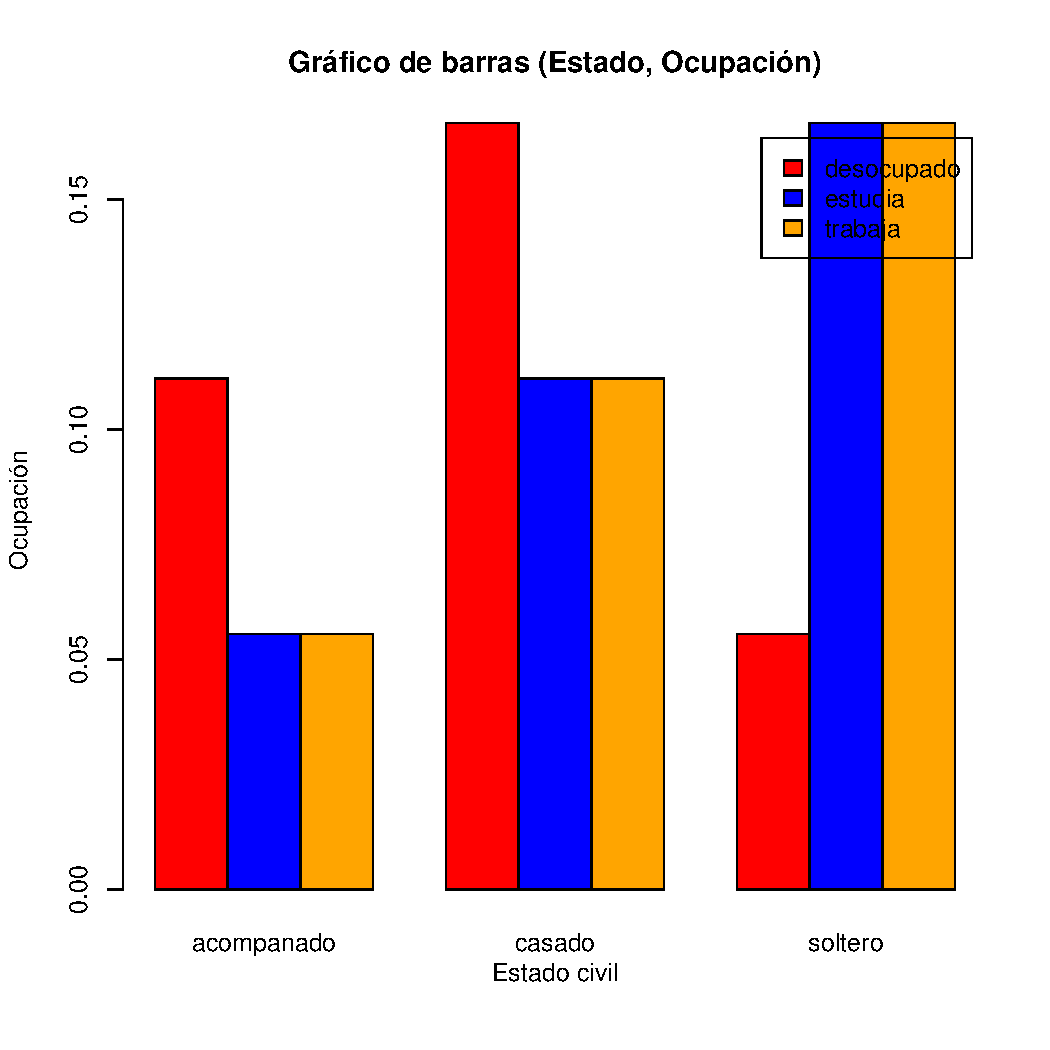
\includegraphics[width=\maxwidth]{figure/unnamed-chunk-15-1} 

\end{knitrout}
\end{enumerate}
\end{document}
